\documentclass[a4paper,12pt]{article}

% \usepackage[utf8x]{inputenc}
\usepackage[T1]{fontenc}
\usepackage[english]{babel}
\usepackage[left=3.5cm,right=2.5cm,top=2.5cm,bottom=2.5cm]{geometry}
\linespread{1.5}
\usepackage{mathptmx}
\usepackage{courier}
\usepackage{amsmath,amssymb}
\usepackage{graphicx}
\usepackage{booktabs}
\usepackage{array}
\usepackage{hyperref}
\usepackage{listings}
\usepackage{xcolor}
\usepackage[style=numeric, sorting=none]{biblatex}
\usepackage{csquotes}
\usepackage{float}

\addbibresource{bibliografia.bib}
\hypersetup{hidelinks}

\lstdefinestyle{mystyle}{
    backgroundcolor=\color{gray!10},
    commentstyle=\color{green!50!black},
    keywordstyle=\color{blue},
    numberstyle=\tiny\color{gray},
    stringstyle=\color{orange},
    basicstyle=\ttfamily\footnotesize,
    breaklines=true,
    numbers=none,
    % numbers=left,
    % numbersep=5pt,
    showstringspaces=false,
    tabsize=2,
    frame=single
}
\lstdefinelanguage{json}{
    basicstyle=\ttfamily\footnotesize,
    numbers=none,
    breaklines=true,
    showstringspaces=false,
    frame=single,
    backgroundcolor=\color{gray!10},
    literate=
     *{0}{{{\color{blue}0}}}{1}
      {1}{{{\color{blue}1}}}{1}
      {2}{{{\color{blue}2}}}{1}
      {3}{{{\color{blue}3}}}{1}
      {4}{{{\color{blue}4}}}{1}
      {5}{{{\color{blue}5}}}{1}
      {6}{{{\color{blue}6}}}{1}
      {7}{{{\color{blue}7}}}{1}
      {8}{{{\color{blue}8}}}{1}
      {9}{{{\color{blue}9}}}{1}
      {:}{{{\color{black}{:}}}}{1}
      {,}{{{\color{black}{,}}}}{1}
      {\{}{{{\color{red}{\{}}}}{1}
      {\}}{{{\color{red}{\}}}}}{1}
      {[}{{{\color{red}{[}}}}{1}
      {]}{{{\color{red}{]}}}}{1},
}
\lstset{style=mystyle}

\author{Claudio Lucisano}
\date{}

\newcommand{\code}[1]{\texttt{#1}}

\begin{document}
\begin{titlepage}
\centering
\textbf{Università della Calabria}\\[0.3cm]
\textbf{Dipartimento di Matematica e Informatica}\\[0.5cm]

\includegraphics[width=0.95in,height=0.6in]{./media/UnicalLogo.png}\\[0.5cm]
\textbf{Corso di Laurea Magistrale in Informatica}\\[1cm]
{\Large Tesi di Laurea}\\[0.5cm]
{\Large \textbf{PABEL: Plugin ABE for LLM}}\\[2cm]
{\large \textbf{Ensuring Document Confidentiality for AI Agents via Attribute-Based Encryption}}\\[2cm]

\begin{tabular}{@{}p{0.5\linewidth}p{0.4\linewidth}@{}}
\toprule
\textbf{Relatori} & \textbf{Candidato} \\
\midrule
Ch.mo Prof. Giovambattista Ianni & Claudio Lucisano \\
Dott. Andrea Altarui & Matricola 231871 \\
\bottomrule
\end{tabular}

\vfill
Anno Accademico 2025/2026
\end{titlepage}
% \newpage
% \begin{abstract}
% AI coding agents send the content of the files they read to a third-party model provider; once data leaves the organization, trusting the agent or the vendor is not a guarantee. This thesis presents PABEL, a system that replaces this trust with cryptography: documents are encrypted with Ciphertext-Policy Attribute-Based Encryption (CP-ABE), section by section, each under its own policy, satisfied only by the combined attributes of the human user \emph{and} of the specific agent acting on their behalf. An MCP server performs all the decryption, Keycloak authenticates the user and identifies every agent installation, and a connector on the employee's machine intercepts the file accesses of the agent through hooks and relays them to the server. The agent never holds keys and receives only the sections its user--agent pair may read. The evaluation compares observed and expected outcomes for every pair, runs attack scenarios derived from the threat model and measures the cost of the interception. It also shows where the guarantees end: after the plaintext is released, and for agents that cannot be intercepted.
% \end{abstract}
\newpage
\tableofcontents
\newpage
\section{Introduction}
\subsection{Context and Motivations} \label{Context and Motivations}
% Descrivere il contesto scientifico e tecnologico in cui si colloca l'attività di tesi e quali sono le motivazioni per lo sviluppo del progetto di tesi. (circa 2 pagine)
The constant and rapid evolution in the field of Artificial Intelligence has result in a day-to-day use of AI agents, thus the need of security and privacy when dealing with tools that, potentially, could harvest personal or company data for a variety of reasons.
More in detail the concept that we were trying to focus on, was the scenario in which an employee, by chance or intentionally, had its AI agent to look at a confidential file which the company doesn't want to be leaked or simply does not trust the AI agent's vendor.

This particular fear, to not trust AI vendors, it's not unfounded; several recent incidents show how sensible data can end up outside the boundaries an organization intended to enforce, or how AI providers themselves may proceed to process user data in ways that raise legitimate concerns.

A well known example is the 2023 Samsung incident, where some employees pasted proprietary source code into a public LLM chatbot for debugging purposes, effectively transmitting confidential IP (intellectual property) to an external, unintended infrastructure. This incident led Samsung to ban all AI tools altogether\cite{samsung2023leak}

A second, more institutional, example involves OpenAI: in december 2024, the Italian Data Protection Authority fined OpenAI for \texteuro15 million, finding that ChatGPT was processing users' personal data to train underlying models without the legal basis required by the GDPR; not to mention a security breach, that took place in march 2023, which exposed users' data and payment information\cite{garante2024openai}.

Also Anthropic was acting in regard of the guarantees that have to be assumed by a vendor, in particular it had to update its customer terms\cite{anthropic2025terms}. They explicitly stated that each conversation made with Claude could be used for model training, with the exception of Claude for Work, Claude Enterprise, Claude Gov and any API-based access\cite{anthropic2025terms}.

These three exapmles share a common thread, that is once data leaves an organization's boundary and reaches a third-party model or vendor, the organization has no further technical control over it. This thesis takes the position that this control should not depend on trusting the AI agent's behavior, nor on trusting the vendor's policies, but should instead enforced cryptographically, when accessing the data.
\subsection{Activities done and Results}
In this thesis, we have designed and implemented a plugin for AI agents that allows to decrypt files using Attribute-Based Encryption (ABE) in order to ensure that only authorized users and authorized AI Agents can access specific parts of the file. The plugin is designed to be easily integrated into existing AI agents, providing a seamless way to enhance security and privacy in AI-driven environments.

Such security enhancement is achieved by encrypting files with ABE, which allows for fine-grained access control based on user and AI agent attributes. PABEL intercepts file access requests from the AI agent, authenticates the user and checks, via server, if both the user's attributes and the agent's attributes match the encryption policy; thus the server decrypts the specific parts of the file that both the user and \emph{that} agent are authorized to see and returns it to the agent.

This approach ensures that sensitive information remains protected when accessed by AI agents, since every sensitive information is handled server-side and the agent does not perform any sort of decryption and does not even hold any cryptographic material needed to do so.

The result is a working end-to-end system: a CP-ABE capable MCP server, an agnostic connector that has been verified against multiple agents and a hardened workflow to ensure agents' identites.
\subsection{Technologies and Tools}
To achieve the goals of this thesis, several technologies and tools have been utilized.
The core of the security mechanism is based on Attribute-Based Encryption (ABE), more in particular we have used the open source library \textbf{OpenABE}\cite{openabe}, which we had to upgrade to a more recent version by updating its dependecies and fixing some bugs that were present in the original code (Section \ref{sec:openabe}).

Another important component of the system is the authentication and authorization mechanism, which is implemented using \textbf{Keycloak}, an open-source identity and access management solution. Keycloak provides a robust framework for managing user identities, roles, and permissions, which is essential for enforcing access control policies in the context of ABE.

The plugin is designed to be compatible with AI agents that support plugin integration, and it has been tested with specific AI agents and harnesses to ensure proper functionality.
The AI agents used for testing are:
% TODO: add more AI agents if needed
\begin{itemize}
    \item \textbf{Claude Code}, an AI agent developed by Anthropic; 
    \item \textbf{Codex}, an AI agent developed by OpenAI;
    \item \textbf{Copilot for VSCode}, an AI agent developed by Microsoft, integrated into the Visual Studio Code IDE.
    \item \textbf{OpenCode}, an open-source AI agent.
\end{itemize}
Throughout the project we used Python as main language, as well as Python libreries such as \textbf{PyJWT}, \textbf{FastMCP} and \textbf{Psycopg}.
The server-side component of the system was containerized using \textbf{Rancher Desktop}, a tool that allows to run Kubernetes clusters on a local machine. This setup enables easy deployment and management of the server component, hence supporting scalability and reliability in handling decryption requests from AI agents.
Alongside the server container, there were deployed two other containers: one for the Keycloak, which contains identities and attributes, server and another for a \textbf{PostgreSQL} database, which (in combination with Keycloak) store agent installation's information and generated keys. This containerized approach simplifies the deployment process and allows for an easy scaling of the system as needed.

\subsection{Thesis outline}
% TODO: ROADMAP
After a description of the motivation and also a security overlay of this work in section \ref{Motivation and Threat Model}, we'll cover some background informations in section \ref{Background}, especially \nameref{ABE}, before heading in a in-depth analysis of the System Design in section \ref{System Design}.
Will follow a Security Analysis in Section \ref{Security Analysis}, alongside some evaluations and the conclusions, respectively, in Sections \ref{Evaluation} and \ref{Conclusions}.

\newpage
\section{Motivation and Threat Model}\label{Motivation and Threat Model}
\subsection{Problem Statement}
% This thesis addresses the security challenges that arise when AI agents are granted access to organizational or sensitive data. In particular, access control should not depend solely on the agent's reasoning capabilities or on its ability to correctly interpret the sensitivity of data.
The main problem that this thesis aims to solve comes from a consideration while thinking how AI can be implemented in a blue team scenario.
Even if this topic could be an argument of discussion by itself, many perplexities arise when we think how data is exchanged considering AI agents actively inside the attack surface.

In particular, the problem is that AI agents are not able to distinguish between sensitive and non-sensitive data and, furthermore, they are not able to understand the context of the data they are processing. This means that if an AI agent is given access to sensitive data, it could potentially leak that data to an attacker, either intentionally or unintentionally.
Of course, it is imperative to also consider the intrinsic vulnerability of AI agents to prompt injection attacks \cite{debenedetti2025defeating}, which could be just another mean to the exfiltration of sensitive data as aforementioned.

One method to mitigate this problem would be to utilize cryptography, but that alone comes with its own set of challenges. More in detail, both an AI agent and a user cannot benefit from data that is encrypted with a symmetric key: both of them would require a decryption of said  data, otherwise they would not be able even to understand it, let alone use it.

One possible alternative could be Homomorphic Encryption and, surely, it is a very promising topic, but as of today its computational limitations make it not suitable for a real-world scenario, especially if we consider the amount of data that an AI agent should process.

Another approach to achieve more security in a scenario that involves a LLM could be Trusted Execution Environments, but here lies the need (thus the problem) to ensure that the AI agent is running in a trusted environment, which is not always possible, especially if we consider that the AI agent could be running on a remote server or in a cloud environment.

Hereby we'll expand on the limitations of both Homomorphic Encryption and Trusted Execution Environments, to better understand and define the problem we are trying to solve.
\subsubsection{Limitations of Homomorphic Encryption}
As aforementioned, Homomorphic Encryption (HE) is a very promising topic, given the ability it enables to perform homomorphic operations on encrypted data. The problems arise when we approach statistical computations, which is the basis of Large Language Models, and, in general, of any AI agent.

Precisely on this regard, \citeauthor{cheon2017homomorphic} eloquently stated \cite{cheon2017homomorphic}:
\begin{quote}
    Most of real-world data contain some errors from their true values. [...] an approximate value may substitute the original data and a small rounding
error does not have too much effect on computation result [...]
    Unfortunately this rounding operation has been considered difficult to perform on HE
since it is not simply represented as a small-degree polynomial.
\end{quote}
They proposed a scheme that allows to perform approximate computations on encrypted data, not without open problems, like the need to convert said scheme in a fully homomorphic scheme using bootstrapping. This problem was later addressed by \citeauthor{de2025encryptedllm} who proposed a GPU-based workflow by extending the capabilities of OpenFHE \cite{al2022openfhe}.

Said implementations is undoubtly a great step forward towards practical encrypted LLM, but it has still non trivial limitations:
\begin{quote}
    Although promising given the massive overheads involved in both LLMs
    and FHE (Fully Homomorphic Encryption), this is still far from practical for real-world usage,
    even for applications that are not latency sensitive such
    as text summarization or content generation (in contrast to
    chatbots or Q/A tasks, which are more demanding in terms
    of responsiveness).
\end{quote}
The main problem is that, even with a GPU-accelerated implementation, the bootstrap overhead (also in combination with the LLM inference overhead) is still too high to be considered practical in a every day scenario.
To this we have to take in account also that by approximating the functions needed to have LLM inference we are introducing a source of error that translates into a loss of accuracy in the final result.
Both of this factors alone make Homomorphic Encryption, as per today, not viable to be used in application such as chatbot or coding agents and it is clear why Attribute-Based Encryption could fill the gap in this point and time by providing security precisely where the FHE, at the moment, cannot provide.
\subsubsection{Limitations of Trusted Execution Environments}
Trusted Execution Environmets, as the name suggests, are trusted environment where it is possible to execute critical operation and, in the context of prompt injection and LLM, potentially separate a network or an entire device from the execution of malicious actions by the agent that, in fact, would only be relegated in a sandbox.

\citeauthor{geppert2022trusted} define TEEs as following:
\begin{quote}
    TEEs [...] are defined as tamper-resistant processing environments that run on a separation kernel.
    Remote verification makes the technology suitable for cloud
    environments. It is a mechanism proving to
    an organization that uses the services of a cloud provider that the
    specified software runs on the predefined hardware even if the
    organization does not have direct access to this hardware.
\end{quote}

In the cloud computing scenario this sort of infrastructure is already offered by providers like Google, Amazon, and Microsoft \cite{geppert2022trusted}, but this would not apply to some organization that don't want to rely on external provider. This is extremely crucial even when talking of LLMs, since if an organization opted to rely on third party agents (i.e. Claude Code, Codex, etc...) it would rely to this third party also all the security assumptions that arise.

To better explain this concept, by considering the use of a TEE provided by some provider, an organization would not have any control on \textit{how} its own data are manipulated. It is obvious that in most cases this is not an acceptable risk and many would resort to a "home-made" solution, like training its own LLM; this issue, although, could be mitigated if we consider a situation where only pre-approved data can be "sent out", thus the application of Attribute-Based Encryption and the not suitability of TEE in every scenario.

Summarizing, even though TEEs \textquote[\cite{han2026automated}]{minimizes potential security issues such as data leakage, unauthorized access, code tampering, and software-based attacks}, they do not take in consideration the cases in which a company does want to fine grain the data that escape the company's domain.
\subsection{Related Works}\label{related}
To the best of our knowledge a few, if not none, of recent works constain what an AI agent may do rather than what it may read.
A few example can be 

\subsection{Actors and Goals}
In this section we define the actors involved in the system and their goals, to better understand the problem we are trying to solve.

The actors, with their own goals, involved in the system are:
\begin{itemize}
    \item \textbf{User:} the user is the person that wants to use an AI agent to process a document. The user has a set of attributes that define their access rights to the document.
    \item \textbf{AI Agent:} the AI agent is the entity that retrieves and processes the document. The AI agent has a set of attributes that define its access rights to the document.
    \item \textbf{Company:} the company is the entity that owns the document and defines the access policy for it, alongside the attributes of the users and the AI agents. The company is responsible for ensuring that the access policy is enforced and that the sensitive data is protected.
    \item \textbf{IT/Cybersec:} the company's departments responsable for the security of the documents (i.e. encrypting, authorizing and auditing) and the company allthoghether
\end{itemize}

\subsection{Assumptions}\label{Assumptions}
We assume that the documents subject to protection are already produced and encrypted via Attribute-Based Encryption before being made available to the system described in this work. Authoring a new document, defining its access policy, ensuring the freshness of employees' attributes, generating the corresponding keys, encrypting the document, are all separate concerns and fall out of the scope of this thesis, which focuses on enforcing, at read time, a mechanism that allows an AI agent to process the document following a safe workflow, minimizing the risk of sensitive data exfiltration.

We also assume that our garantees end at the moment decrypted content is legitimately handed to the requesting AI agent, in accordance with the CP-ABE policy and the combined attributes of the user and the agent.
What the agent does with that content afterwards is not something an access-control layer, operating at application level, can control and it is, therefore, out of scope. There is an exception worth to mention, that is locally materialized copies which are time-bounded and removed automatically at the end of a session, to limit possible unbounded exposure.

By design, the system assumes that the encrypted documents are \code{.abe} files, that is they carry a predefined structure (as defined in Section \ref{File Structure}) that can be read without decrypting them and are recognised by their extension.

\subsection{Adversary Model}
In this section we'll describe what entities are considered as adversary.
By default, we assume the worst case scenario: both AI agent and its Vendor are not trusted, nor the user itself.
Mainly, we can differentiate three different threat entities:
\begin{itemize}
    \item \textbf{AI agent / Vendor:} the agent itself can be "too curious", it can be compromized or worse, its vendor can actively try to use customer data for its own goals (see \ref{Context and Motivations}). It's important to assume the worst case scenario, and to don't trust the model.
    \item \textbf{User:} both by error and intentionally, a user could try to use its AI agent to read something outside the user's authorization level.
    \item \textbf{Attacker:} an external entity that could also intercept traffic data and, possibly, forge malicious content.
\end{itemize}
It is imperative to understand and prevent possible data leaks, hence our proposal to put at risk only a certain part of confidential data (choosen by the company or who possess them).

It's also important to note that there are goals outside this work's scope such as:
\begin{itemize}
    \item \textbf{OS/Endpoint already compromised:} if an attacker has already access to the machine, it is quite easy to see how this system cannot ensure its premises.
    \item \textbf{Secure storage of CP-ABE master key:} the CP-ABE master key is assumed to be protected by the company through appropriate measures to store it safely; its compromise would void every guarantee of the system.
    \item \textbf{Agent behaviour post reception of confidential data:} it is impossible for this system to control what an agent will do to a file once recieved. After the reception of the file, adequatly decrypted, it is responsability of the user what will happen to the data.
    \item \textbf{DoS attacks:} this system does not guarantee the availability, but the adequate confidenciality of data.
\end{itemize}
\subsection{Security Goals}
The end goal of this work is to provide a simple way to handle sensitive data with a fine-grained access control enforced by a company, such that its own employee could not provide leaks whenever they use an AI agent beyond their authorization, since the access control mentioned above.
This allow also to audit each and every operations on encrypted files, that is offering an invaluable tool for Cybersec/IT departments, which could easily track any eventual misbehaviour.

Our work certainly benefit corporate environments, but also any enviornment where it is wanted to limit what agents can see and therefore where more controlled access is needed, whit a consequent help on data leak control.
\newpage
\section{Background}\label{Background}
\subsection{Attribute-Based Encryption}\label{ABE}
Attribute-Based Encryption, as the name suggest, is a type of encryption that enforce an access control via attributes and authorization policies. The secret key of a user and the ciphertext are both dependent by attributes.

First proposed as a concept in 1984, it was improved and implemented in the first years of 2000s; it presents two main types of encription schemes: the \textbf{key-policy attribute-based encryption (KP-ABE)} \cite{goyal2006attribute} and the \textbf{ciphertext-policy attribute-based encryption (CP-ABE)} \cite{bethencourt2007ciphertext}.

\subsubsection{From Identity-Based to Attribute-Based Encryption}
Identity-Based Encryption is a type of public key cryptography based on PKI (Public-Key Infrastructure), with the main difference being the fact that IBE allows a 1 to 1 relationship between sender and reciever.
As \citeauthor{shamir1984identity} said in his paper \cite{shamir1984identity}:
\begin{quote}
    The scheme is based on a public key cryptosystem with an extra twist: Instead of generating a random pair of public/secret keys and
publishing one of these keys, the user chooses his name and network address
as his public key. Any combination of name, social security number, street address, office number or telephone number can be used (depending
on the context) provided that it uniquely identifies the user
in a way he cannot later deny, and that it is readily available to the other party.
\end{quote}
The signature scheme abide the following verification condition \cite{shamir1984identity}:
\begin{equation}
    s^e = i \cdot t^{f(t,m)} \mod{n}
\end{equation}
Where 
\begin{itemize}
    \item $m$ is the message,
    \item $s,t$ is the signature,
    \item $i$ is the user's identity,
    \item $n$ is the product of large primes,
    \item $e$ is a large prime reltively prime to $\phi(n)$,
    \item $f$ is a one way function.
\end{itemize}

IBE applications are quite immediate to understand, for example, the ability to ensure that only a given person could read a message, without relying on the PKI, is quite remarcable. There is, anyway, a trust assumtpion towards the Private Key Generator (PKG), which if compromised would nullify the secrecy of every encrypted data that use its issued keys.

Besides, IBE did point towards ABE; we can see how \citeauthor{sahai2005fuzzy} already introduced an ABE approach while proposing a Fuzzy Identity-Based Encryption. They did note how a system where an authority gave a user different keys for each of the attributes that describe the user could easily fall prey of collusion attacks, where multiple users combine their keys to form identities, with a combination of said attributes, that could decrypt ciphertext which none of the individual user could be able to decrypt alone \cite{sahai2005fuzzy}.
This occurs by considering an identity as a set of attributes and, precisely for that, FIBE for the first time achieved error tolerance; it allows for a private key for an identity, say $\omega$, to decrypt a ciphertext encrypted with an identity $\omega'$ if and only if $|\omega \cap \omega'| \geq d$, where $d$ is fixed during the setup and indicates the error tolerance threshold.

\citeauthor{goyal2006attribute}, later proposed a better implementation that was further expanded by \citeauthor{bethencourt2007ciphertext}, de facto introducing, respectively, KP-ABE and CP-ABE.
\subsubsection{Ciphertext-Policy versus Key-Policy ABE}\label{CPvsKP}
The main difference between KP and CP ABE is their approach to the policy needed to decrypt.
While in the Key-Policy ABE the key holds the policy for the identity, in the Ciphertext-Policy ABE is the ciphertext that holds said policy.
In other words, for a KP approach, think of a company that encrypt all its mails with the headers as attributes, say\\
\noindent
\code{\{reciever: developers, object: project-x, date: 20-dec\}}
\noindent\\
When an analist, for a given reason, has to read those mails it will recieve a new key suited for the occasion, for example:\\
\noindent
\code{(reciever=developers AND object=project-x) OR (date>20-dec)}
\noindent\\
This key and this key alone can decrypt the mails that satisfy the key's rule.

Using CP ABE, instead, shift the policy on the document itself: for example, always in a corporate environment, the company encrypted a reserved memo already knowing who can read it, thus it encrypted the document with a policy like:\\
\noindent
\code{(department=finance) OR (management AND security\_level > 5)}
\noindent\\
With this setup only those employees who are in the finance department or are in management, with a security level greater than 5, can access this document. In summa, the paradigm shift from the rule attached to the reader (KP-ABE) to the rule attached to the document (CP-ABE).

Both KP and CP, however, share the definition of a collusion resistant structure, an \textbf{Access Structure}, and four fundamental algorithms: \textbf{Setup}, \textbf{Encrypt}, \textbf{Key Generation} and \textbf{Decrypt} \cite{goyal2006attribute,bethencourt2007ciphertext}.
Moreover, those implementations differ on \textbf{Encrypt}, \textbf{Key Generation} and \textbf{Decrypt}, furthermore, CP ABE includes also a \textbf{Delegate} algorithm. It is all defined as:
\begin{itemize}
    \item \textbf{Access Structure:} Let ${P_1, P_2, ..., P_n}$ be a set of parties. A collection $A \subseteq 2^{P_1, P_2, ..., P_n}$ is monotone $if\ \forall\ B,C\, :\, if\ B \in A\ and\ B \subseteq C\ then\ C \in A$. An \textbf{Access Structure} (monotone access structure) is a collection (monotone collection) $A$ of non-empty subsets of ${P_1, P_2, ..., P_n}$, i.e. $A \subseteq 2^{P_1, P_2, ..., P_n} \setminus {\emptyset}$. The sets in $A$ are called the authorized sets, and the sets not in $A$ are called the unauthorized sets.
    \item \textbf{Setup:} takes no input other than the implicit security parameter. It outputs the public parameters $PK$ and a master key $MK$.
    \item \textbf{KP Encrypt:} a randomized algorithm that takes as input a message $m$, a set of attributes $\gamma$, and the public parameters $PK$. It outputs the ciphertext $E$.
    \item \textbf{KP Key Generation:} a randomized algorithm that takes as input an \textbf{Access Structure} $A$, the master key $MK$ and the public parameters $PK$. It outputs the decryption key $D$.
    \item \textbf{KP Decryption:} takes as input the ciphertext $E$, encrypted under the set $\gamma$ of attributes, the decryption key $D$ for access structure $A$ and the public parameters $PK$. It outputs the message $M\ if\ \gamma \in A$.
    \item \textbf{CP Encrypt:} takes as input the public parameters $PK$, a message $M$, and an access structure $A$ over the universe of the attributes. The algorithm encrypt $M$ and produce a ciphertext $CT$ such that only a user that possesses a set of attributes that satisfies the access structure will be able to decrypt the message. It is assumed that the ciphertext implicitly contains $A$.
    \item \textbf{CP Key Generation:} takes as input the master key $MK$ and a set of attributes $S$ that describe the key. It outputs a private key $SK$.
    \item \textbf{CP Decryption:} takes as input the public parameters $PK$, a ciphertext $CT$, which contains an access policy $A$, and a private key $SK$, which is a private key for a set $S$ of attributes. If $S$ satisfies $A$ then the algorithm will decrypt $CT$ and return the message $M$.
    \item \textbf{CP Delegate:} takes as input a secret key $SK$ for some set of attributes $S$ and a set $\tilde{S} \subset S$. It outputs a secret key $SK$ for the set of attributes $\tilde{S}$. 
\end{itemize}
In summary, we can summarize the main difference between KP-ABE and CP-ABE in a single question: \textit{who decides who can read the document, the party that encrypts it or the party that issues the keys?}
With KP-ABE the policy is embedded in the user's key, so it is fixed by the key issuer and whoever encrypts the document can only label it with attributes, with no means to control who will be able to read it.
With CP-ABE, instead, the policy is embedded in the ciphertext, hence the decision belongs to whoever encrypts the document.

Given that in PABEL the document owner must define who can read the document at encryption time, CP-ABE is the natural choice and, in fact, it is the scheme adopted in the rest of this work.
Moreover, even if both approaches are collusion resistant (i.e. a user with attribute "finance" and another one with "management" cannot decrypt together something that they could not read alone), the well-known limits that CP-ABE implies are a good fit for our system and actually turn out to be consistent with our setting.

First, the policy is fixed when the document is encrypted. This is acceptable here because a given policy expresses a decision taken beforehand by the company: changing it requires re-encrypting the document, an operation that neither a user nor an agent can perform. Since the decryption is not performed client-side, it also shifts the computational overhead entirely to a server.

Second, the policies being monotone, which means \textit{access can only be granted and never subtracted by a negation}, is a deny-by-default behaviour that works perfectly in a scenario in which we want to \textit{specify who is permitted to read specific information}. Basically, anything that falls out of the scope prior defined by the document's owner is denied. This follows tha same reasoning behind a whitelist firewall, which is generally considered safer than a blacklist one: a blacklist \textit{must} anticipate every possible threat, so whatever is not foreseen is allowed, whereas a whitelist enumerates only what is legitimate, hence whatever is not foreseen is blocked.

Third, revoking keys is notoriously hard, but in our system neither the user nor the agent ever holds one: keys are kept server-side, so revoking an agent is litterally a matter of deleting a database entry or updating it with a "revoked" flag.

Finally, CP-ABE relies on a single central authority that holds the master key; for a company that needs a single point of control and auditing, this is a feature rather than a drawback, although it places the server inside the trusted computing base.
\subsection{Identity and Access Management}
Identity and Access Management (IAM) is a set of processes and technologies that establish \textit{who} is making a request (authentication) and \textit{what} that party is allowed to do (authorization), keeping both decisions in a single, auditible place.
A modern IAM typically provides a single sign-on (SSO), multi-factor authentication and a central directory of users together with their attributes (e.g. department, role, etc...).

\begin{figure}[h]
  \centering
  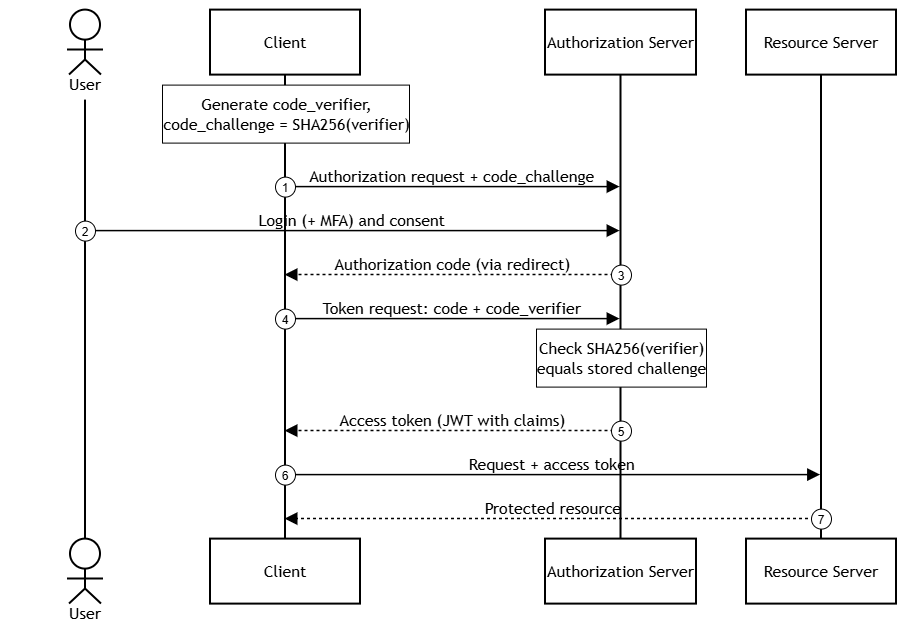
\includegraphics[width=\textwidth]{media/diagrams/IAM.png}
  \caption{A typical IAM flow}
\end{figure}

This last point is the one that matters the most for this work. In CP-ABE the capabilities of a user are entirely described by its attributes, so whoever is the authoritative source of those attributes is, de facto, the one deciding which key can exists.
Delegating this role to an IAM means that attributes are not self-declared by the user or by the agent, but asserted by a trusted party and carried in a token.
The same idea underlies attribute-based access control in general, where the authorization to perform an operation is determined by evaluating the attributes of the subject against a policy \cite{nist800162}.
\subsubsection{OAuth 2.0 and PKCE}
OAuth 2.0 is an authorization framework that allows a client application to obtain limited access to a resource on behalf of a user, without ever handling the user's credentials: it is used, instead, an \textit{access token}, which denotes a specific scope and lifetime \cite{rfc6749}.
The user authenticates against an authorization server, which issues the token to the client; the token is then presented to the server that exposes the protected resource. Tokens are often encoded as JSON Web Tokens (JWT), a compact format for representing claims between parties that can be digitally signed \cite{rfc7519}
Is it through such claims that user attributes can travel from the IAM to the other parts of the system.

In the Authorization Code flow the client first receives a temporary \textit{authorization code} through a redirect and then exchanges it for a token. For public clients, such as command line tools or mobile and desktop applications, this code can be intercepted by a malicious application on the same device and the client has no safe place to store a secret that would prevent its use \cite{rfc7636}.
Proof Key for Code Exchange (PKCE) closes this gap by generating a random \textit{code verifier} for each client's request and sends only its trasformation
\begin{equation}
    \texttt{code\_challenge} = \mathrm{BASE64\_URL}\big(\mathrm{SHA256}(\mathrm{ASCII}(\texttt{code\_verifier}))\big)
\end{equation}
with the authorization request, then discloses the verifier itself only when redeeming the code \cite{rfc7636}.
An attacker who steals the code will not know the verifier and, since the use of SHA-256 as a one-way function, cannot derive it from the challenge.

Although PKCE was originally designed for native applications, is current best practise to use for all kinds of OAuth clients, including confidential ones \cite{rfc9700}.
\subsubsection{Keycloak}
Keycloak is an open-source IAM based on standard protocols. It supports OpenID Connect, OAuth 2.0 and SAML.
At its core there are these concepts:
\begin{itemize}
    \item \textit{realm:} manages a set of user, credentials, roles and groups;
    \item \textit{client:} an entity that can request to authenticate a user;
    \item \textit{protocol mapper:} it allows to select which claims are stored in the issued tokens.
\end{itemize}
Keycloak does also support one-time password (OTP), such as Time-based OTP (TOTP) and HMAC-based OTP (HOTP) through FreeOTP.
We chose it because of its open-source nature, to being consistent with the assumption of an organization who does not want to rely on third parties.
\subsection{The Model Context Protocol}
\blockcquote{mcpspec}{Model Context Protocol (MCP) is an open protocol that enables seamless integration between LLM applications and external data sources and tools.}

It uses JSON-RPC 2.0 messages to establish communication between:
\begin{itemize}
    \item \textbf{\textit{Hosts:}} LLM applications that initiate the connection
    \item \textbf{\textit{Clients:}} Connectors within the host
    \item \textbf{\textit{Servers:}} Services that provide context and capabilities
\end{itemize}
More specifically, servers can offer to clients
\begin{itemize}
    \item \textbf{\textit{Resources:}} Context and data, for the user or the AI model to use
    \item \textbf{\textit{Prompts:}} Templated messages and workflows for users
    \item \textbf{\textit{Tools:}} Functions for the AI model to execute
\end{itemize}
And clients may offer, on the other end, \textbf{\textit{Elicitation}}, that is server-initiated requests for additional information from users.

However, in any situation, since the powerful capabilities through arbitrary data access and code execution, an implementor \textit{must} carefully address \textbf{user explicit consent and} persistent \textbf{control} over what data is shared; \textbf{data privacy}, taking the appropriate measures, and ensuring that hosts must obtain explicit user consent before exposing data to servers; last, but not least, \textbf{tool safety}, since every tool represent an \textit{\textbf{arbitrary code execution}}.

For our purposes, MCP provides not only a resource server, but also the legitimate channel through which the agent asks for a document: the server owns the decryption logic and returns only the content that the policy allows. The idea is to offer to agents a black box to interact with, so they would never handle sensitive informations or at least they would not be capable to retrieve what it is not them permitted.
\subsection{Hook-Based Interception in AI Coding Agents}
Many coding agents expose \textbf{\textit{hooks}}, i.e. user-defined command that the agent's runtime execute at precise points of its lifecycle, such as before a tool call (\code{PreToolUse}), which can also block the call \cite{claudehooks,copilothooks}.
In Claude Code, for instance, the hook receives the description of the event as JSON on standard input (tool name and arguments) and answers with a decision: allow the call, deny it with a reason, rewrite its input (\code{updatedInput}) or add context for the model (\code{additionalContext}).

The crucial property is where the hook runs. An instruction written in a prompt or in a \code{skill} is only text that the model reads: it may be ignored, misinterpreted or even overridden by a prompt injection \cite{debenedetti2025defeating}, so it cannot be a security control.
A hook is, instead, executed at runtime \textit{outside} the model's reasoning, hence its decision does not depend on the model's cooperation. This is why \textbf{we implement enforcement as a hook} and use \textbf{skills}, informationally, \textbf{only to explain to the agent \textit{why} a read was replaced}.

Hooks are however not uniform across vendors. Copilot CLI, for example, documents a similar \code{preToolUse} event with a \code{permissionDecision} field, but it names the field that rewrites the arguments differently (\code{modifiedArgs}) and supports both camelCase and PascalCase formats \cite{copilothooks}.
Moreover, some channels are not reliably delivered in practise (see the adapters in Section \ref{System Design}). This heterogenity motivtes the per-agent adapters of our design.

\newpage
\section{System Design}\label{System Design}
\subsection{The OpenABE Library}\label{sec:openabe}
The cryptography used in PABEL is provided by OpenABE \cite{openabe}, an open-source C/C++ library that implements ciphertex-policy and key-policy ABE together with command-line tools used for key generation and decryption.

The upstream version (v 1.0.0), last updated in May 2023, is written in C++11 and depends on OpenSSL 1.1.1 and RELIC 0.5.0.
It was necessary an upgrade of those dependency since, trying to building it on Windows, many errors occurred, from installation ones to logic ones.
Therefore we ported the library to OpenSSL 4.0.1, RELIC 0.7.0 and C++17, thus making available a build on Windows (MSYS2) and on the Ubuntu image on the server.

Said port is released as a fork \cite{openabefork} under the same AGPL-3.0 license, where small bugs found along the way were fixed with also contributions made from the community, which we sentitely appriciate. 

\subsection{Architecture Overview}
Our system is composed by two main component:
\begin{itemize}
    \item \textbf{server-side components:} the components include Identity and Access Management (\textbf{Keycloak}), database (\textbf{Postgres}), MCP server that handles logic (with \textbf{OpenABE}).
    \item \textbf{client-side connectors:} adapter and hook grant connection and control over the AI agent.
\end{itemize}
The server-side components are designed to be each one indipendent from the others; we have containerized each one of them with \code{containerd} and made them available with Rancher Desktop.

Client-side there are two parts essential to the correct flow of the program: there is an adapter for each agent and a hook that is the real intermediary between the server-side and the agent.
\subsection{Early Prototyping}
The system did not start in its current form. Before PABEL, the work went through an early prototype that had to answer "how to keep several parts, each with its own policy in a single file" and "how to let a person read and edit that file according to their attributes".
The prototype is described here because it produced the format used throughout this work and because some ideas that PABEL lather adopted, such as the identity coming from Keycloak and a first hook that blocks the direct read, were tried in it first.

\subsubsection{File Structure} \label{File Structure}
To start approaching the concept, it is imperative to subdivide the problem into smaller ones. The first problem that came to mind was to find a way to have into a single file multiple parts, each with its own encryption.
To solve this problem, we did create a JSON structure that could contain each encrypted section of the file, i.e. an array containing a single object per section that has two properties: the policy requested to decipher the ciphertext and the ciphertext itself.
\begin{lstlisting}[language=JSON, caption={.abe format v1}]
{
  "format": "abe-doc",
  "version": 1,
  "sections": [
    {
      "policy": "livello = x",
      "chiphertext": CIPHERTEXT_Lx
    },
    {
      "policy": "livello = y",
      "chiphertext": CIPHERTEXT_Ly
    },
    {
      "policy": "livello = z",
      "chiphertext": CIPHERTEXT_Lz
    }
  ]
}
\end{lstlisting}
It's quite easy to point out that this implementation is very inefficient when the number of sections grows. To optimize the amount of operations needed and the structure of the document itself, it was improved in the version 2 of the structure:
\begin{lstlisting}[language=JSON, caption={.abe v2}]
{
  "format": "abe-doc",
  "version": 2,
  "sections": [
    {
      "group": 0
    },
    {
      "group": 1
    },
    {
      "group": 2
    },
    {
      "group": 1
    },
    {
      "group": 0
    }
  ],
  "groups": [
    {
      "policy": "livello >= 3",
      "ciphertext": CIPHERTEXT_L3
    },
    {
      "policy": "livello >= 2",
      "ciphertext": CIPHERTEXT_L2
    },
    {
      "policy": "livello >= 1",
      "ciphertext": CIPHERTEXT_L1
    }
  ]
}
\end{lstlisting}
This structure provides one key feature: the ability to call the decrypt function $n$ times, where $n$ is the number of unique policies used to rules the sections. This is a more sustainable approach than v1, since, in that case, the decrypt function would be called exactly $m$ times, where $m$ is the amount of each section in the document. It's a fair assumption to say that $m$, \textit{usually}, is greater than $n$.
\subsubsection{From a Viewer to ABEditor}
PABEL only decrypts, so the server never encrypts and, as stated in the assumptions (see \ref{Assumptions}), authoring a document is a taks demanded to whoever uses this system.
To test it, however, there had to be a tool that produced documents with controlled policies and that showed what each identity should see.
That tool started to be implemented as a simple viewer, later evolved together with the rest of the work until it became ABEditor, an application meant for said third party and never installed on a client machine. The following table \ref{tab:editor} summarize its stages:

\begin{table}[htbp]
  \centering
  \begingroup\linespread{1.0}\small
  \begin{tabular}{@{}>{\raggedright\arraybackslash}m{0.24\textwidth}>{\raggedright\arraybackslash}m{0.36\textwidth}>{\raggedright\arraybackslash}m{0.30\textwidth}@{}}
    \toprule
    \textbf{Stage} & \textbf{Problem} & \textbf{Result} \\
    \midrule
    Command-line scripts & verify CP-ABE and numeric hierarchy on a text with section markers & one ciphertext per section, three demo users with keys in files \\
    \code{.abe} v1 and v2 & decryptions grow with the number of sections & one ciphertext per disticnt policy \\
    Graphical viewer & read and edit a document as a given user & open, edit and save a \code{.abe} file \\
    Keycloak identity and first service & use the identity of a real user and let an agent read & keys created in advance and kept in a local keystore, an MCP server with three read-only tools returning every section \\
    First hook & prevent the agent from reading the file directly & direct reads blocked and redirected to the MCP tool \\
    Policy checker & a mistyped policy failed only later, during the encryption & syntax check mirroring the OpenABE grammar \\
    Re-encryption by the authority & change the policy of sections that no local key can read & throwaway key from the master secret key, deleted afterwards, audited \\
    Protected PDFs & realistic documents are PDFs & regions with their own policy over a public layout \\
    \bottomrule
  \end{tabular}
  \endgroup
  \caption{The stages of ABEditor}\label{tab:editor}
\end{table}
The fourth and fifth stages are the core of PABEL. In that early stage, the keys were created beforehand with the authority of the viewer and read by the service, thus a change of attributes in Keycloak required to create the key again by hand.

\subsection{ABEditor: the Authoring Tool}\label{ABEditor}
\subsubsection{Why it is Needed for Testing}
In summary this editor was needed for three principal reasons:
\begin{itemize}
  \item \textbf{Purpose-build documents:} PABEL itself cannot produce documents and there was the need to being able to create a document with multiple policies avoiding an "all or nothing" outcome.
  \item \textbf{Oracle:} A test needs an expected result that does not come from the system being tested, otherwhise a mistake of the system would be repared in the expectation. Hence the editor provides it as an oracle for the needed tests.
  \item \textbf{Controlled variation:} We had to make sure that in an encrypted document every section and distinct policy could be varied indipendently of each other; thus the editor allowed us to produce and edit such documents.
\end{itemize}

\subsubsection{What it does Today}
ABEditor checks every policy before the encryption and can change the policy of a section, even one the selected key cannot read, since it requires the master secret key to operate.
A PDF can be protected by drawing regions, each with its own policy over a public layout from which the content of the regions has been removed and not covered.
The part of the page outside the regions is readable by anyone holding the file and the copies exported to a reader of the system are plain PDFs that no longer have any protection.

\subsection{CP-ABE Authority and Key Management}\label{CP-ABE Authority and Key Management}
It is clear that we have to have a central autorithy that could audit and grant accesses to documents. This operation is made by conjuncting both \textbf{Keycloak} and \textbf{Postgres}:
While \textbf{Keycloak} holds the informations of every user (e.g. mail, department, security level, etc...) and so their attributes, \textbf{Postgres} holds the registry of the allowed agents and the keys in use, one for each pair of user and agent; those attributes are, then, merged in a single key, which is the one the server uses to decrypt.

The concept is simple: after the server has verified the tokens of user and agent, it takes the resultant key of that pair from the database and uses it with \textbf{OpenABE} to serve the decrypt file.
With this solution nobody needs to have installed its own key and it is strictly handled "in background", to both minimizing the risk of tampering and also to ensure a strict control over the allowed agents (it's easy as deleting a row in a db to disable entirely an agent from being used).

\subsection{Human Identity via Keycloak}
Obviously, the Keycloak login can be used with two-factor-authentication (it can also enforce a biometric login). The 2FA itself is out of this scope, but we mention \textbf{FreeOTP} as a free tool used for an otp testing and aswell it is strongly suggested that a MFA (Multi Factor Authentication) is used.

Once the user is logged in, and we can assume it is authenticated, then we can proceed to concede a token which contains the relevant attributes and those will be used to create the key of said user.

\subsection{Agent Identity Model}\label{Agent Identity Model}
In the adversary model of this work the AI agnet is not trusted, so a policy that mentions the agent cannot rely on anything the agent declares about itself.
The identity of the agent \textit{must} be established the same way as the identity of the human, that is by a credential that the agent cannot forge, verified by the server on every call.

\subsubsection{What is Identified: Harness, Surface and Model}
Three different things are usually called \textquote{the agent}:
\begin{itemize}
  \item \textbf{Harness:} the product that owns the tool-call loop and decides whether a file read happens (e.g. Claude Code, OpenCode)
  \item \textbf{Surface:} it is where the harness runs (a terminal, an IDE extension, a desktop application) and only changes where configuration files live
  \item \textbf{Model:} it is what reasons inside the harness (e.g. Sonnet, GPT, etc...)
\end{itemize}
PABEL identifies the harness and nothing else: it never sees the model, and no policy can name it. A clause naming a given harness is satisfied by an installation of that harness regardless of which model is running in it, and is not satisfied by a different harness driving the same model.
The unit of trust is therefore the installed product plus the person using it.

It is important to notice how the enumeration of the model and the surface of an agent is a challenge by itself.
It is also important to remind that PABEL operates at layer 7, thus the impossibility to have an exact picture of what is running on the system; this could be theoretically achieved by implementing an enforcement at OS level.
\subsubsection{Per-Installation Credentials}
Each installation of a harness on a user's machine is registered by an administrator and receives its own Keycloak client, which needs to be authenticated with the OAuth 2.0 \code{client\_credentials} grant.
The \code{client\_secret} is shown once at creation and handed over to the employee out of band. The credential is never reused across two harnesses: sharing it would give them a shared identity, which is exactly what this model prevents.

On every call the server verifies the agent token as it does for the human one (signature, issuer and expiration) and then resolves the identity through a chain that starts from a value that the caller cannot choose:
\begin{enumerate}
  \item the \code{azp} (authorized party) claim of the token, i.e. \code{client\_id} that obtained it, stamped by Keycloak at issuance;
  \item the matching \code{agent\_installations} row, confirming that the installation exists and has not been revoked;
  \item the row of the \code{agents} table of the product it belongs to, which tells wheter the product is enabled, which attribute it contribuites (e.g. \code{agent\_claude\_code}, \code{agent\_opencode}) and which role a user must hold to use it.
\end{enumerate}
The \code{agent\_id} comes out of this chain only after the token has been verified: it is never a parameter of a request, so no caller can claim one.

Keycloak roles are very important and useful to handle specifically \textit{who} can use \textit{what}; someone without the role \code{agent\_claude\_code\_user} could not integrate the agent's attributes, i.e. policies that enforces \code{agent\_claude\_code} would fail.
\subsubsection{Authorization of the Pair}
There are two main types for a request denial when trying to authorize an agent.
\begin{itemize}
  \item An \textit{hard error} is considered whenever there is an invalid (or expired) token or when it is present an unknown or revoked installation and a disabled product, hence the request is simply denied.
  \item A \textit{soft error} present itself if the installation is valid, but the user doesn't hold the role that the product requires (e.g. \code{agent\_claude\_code\_user}); the failure, in this case, resolves in the agent that contributes with no attribute at all. The same user is still authenticated, but any policy that names the agent will fail, so no special deny logic is required: not holding the role \textit{is} the denial.
\end{itemize}
So, whereas there is no \textit{hard error}, the attributes of the user and the one of the agent are then merged togheter in a single CP-ABE key (see Section \ref{CP-ABE Authority and Key Management}).
A section sealed under a policy such as \code{sales and agent\_claude\_code} will open only for someone holding \code{sales} \textbf{\textit{and}} working through a registered Claude Code installation; changing either half keeps the section closed.

\begin{figure}[H]
  \centering
  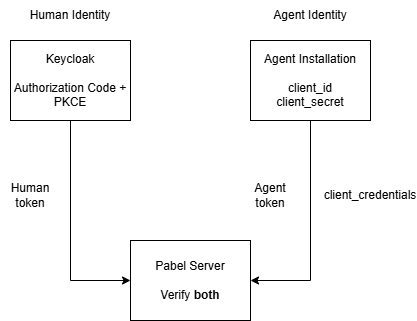
\includegraphics{media/diagrams/Dual Verification Human-Agent.png}
  \caption{The two identities verified by the server on every request}
\end{figure}
\subsubsection{Where the Identity Comes From and its Limits}
Starting from this section an harness with hooks is assumed (the others are discussed in Section \ref{Two Classes of Agents}). As previously mentioned, the agent never holds its own token but it's the hook, instead, that injects the credential of the installation into the call (later expanded in \nameref{The Relay Hook}); the model does not need it and cannot read it.
The strength of this identity is, however, bound to the protection of the credential store on the employee's machine. Whoever can read it can authenticate as that installation from anywhere; this is the compromised-endpoint scenario that is declared out of scope in the threat model.
\subsection{Audit Logging}
Each and every operation the agent make while calling the server is logged, both to track every access to each document and to make every user's accountability verifiable.
Server-side it is all kept in a \code{audit.jsonl}, for semplicity's sake, but it can be enhanced (see \nameref{Future Development}).


\subsection{Connector Architecture}
The shared core evaluates every tool call against the checks of Table \ref{tab:decide} in the order shown, and the first one that applies decides.
Every outcome is also written to a local log (previous installation of a public key for auditing) on the client machine and the denials that would otherwise never reach the server are reported in it, so that it is kept an audit trail.

\begin{table}[htbp]
  \centering
  \begingroup\linespread{1.0}\small
  \begin{tabular}{@{}>{\raggedright\arraybackslash}m{0.3\textwidth}>{\raggedright\arraybackslash}m{0.34\textwidth}>{\raggedright\arraybackslash}m{0.30\textwidth}@{}}
    \toprule
    \textbf{Check} & \textbf{Decision} & \textbf{Why} \\
    \midrule
    The call targets the local credential store & \code{DENY\_CREDENTIAL\_ACCESS} & secrets are used only by the connector's own code \\ \hline
    A command references the connector's internals & \code{DENY\_HOOK\_BYPASS} & the hook is the only sanctioned way to run it \\ \hline
    Direct call to the local PABEL tools & \code{ALLOW} & sanctioned call \\ \hline
    Direct call to the deployed server's tools & \code{ALLOW}, agent token injected & the model never holds the credential \\ \hline
    Write to a protected document & \code{DENY\_MUTATING} & PABEL has no authoring path \\ \hline
    Write to the hook configuration & \code{DENY\_CONFIG\_TAMPER} & it would let the installation act as another agent \\ \hline
    Write to any other file & \code{ALLOW} & writes never reach the relay: only reads and commands do \\ \hline
    Command invoking the OpenABE binaries & \code{DENY\_OABE\_BINARY} & it would bypass the combined key and the audit \\ \hline
    No protected target is mentioned & \code{ALLOW} & not a PABEL concern \\ \hline
    Ambiguous target (directory, pattern, several files) & \code{DENY\_AMBIGUOUS} & it cannot be relayed automatically \\ \hline
    One protected file & \code{DENY\_WITH\_RELAY}, or \code{DENY\_AUTH\_ERROR} / \code{DENY\_RELAY\_ERROR} on failure & the direct read is replaced by the server's result \\
    \bottomrule
  \end{tabular}
  \endgroup
  \caption{Decisions of the shared core, in evaluation order}\label{tab:decide}
\end{table}

\subsubsection{The Relay Hook}\label{The Relay Hook}
Blocking a read of a protected document would be safe but it would imply that the agent would simply be unable to work with it.
The relay hook, instead, \textit{replaces} the blocked read with the access-controlled result of the server, so the agent see the outcome as a normal answer in which some sections may be denied.

The flow of Figure \ref{fig:relay} applies when the shared core finds exactly one protected file in the call (i.e. the last row of table \ref{tab:decide}).
A file is recognised by its \code{.abe} extension first, so that it is protected whenever it is mentioned.

The flow can be summarized in these steps:
\begin{enumerate}
  \item The hook is fired when a request contains a \code{.abe} file.
  \item It attaches two credentials to the request, neither of which is visible to the model. The first one is the human session and the second one is the installation token.
  \item If there is no valid human session, the hook itself starts the interactive browser login, retrying once. The login itself is hosted by Keycloak and if it fails both tries, the request is denied.
  \item The server verifies both tokens, merges the attributes into a single key and decrypts each group. It return \textit{every} section of the document, each one either in plaintext or as \code{[ACCESS DENIED]}; this way the shape of the document is maintained and it is the same for every caller (no impactful analysis can be done on the size of the network packet).
  \item The hook returs a denial of the original read whose content is the result of the server. The adapter writes it in the channel of the specific harness (Table \ref{tab:channels}), thus giving it to the model instead of the file.
\end{enumerate}
Every failure along the way (no authentication, unreachable server, error of the relay) ends in a denial with a message and never in a direct read, thus ensuring that the agent would not reason on it.

\begin{figure}[H]
  \centering
  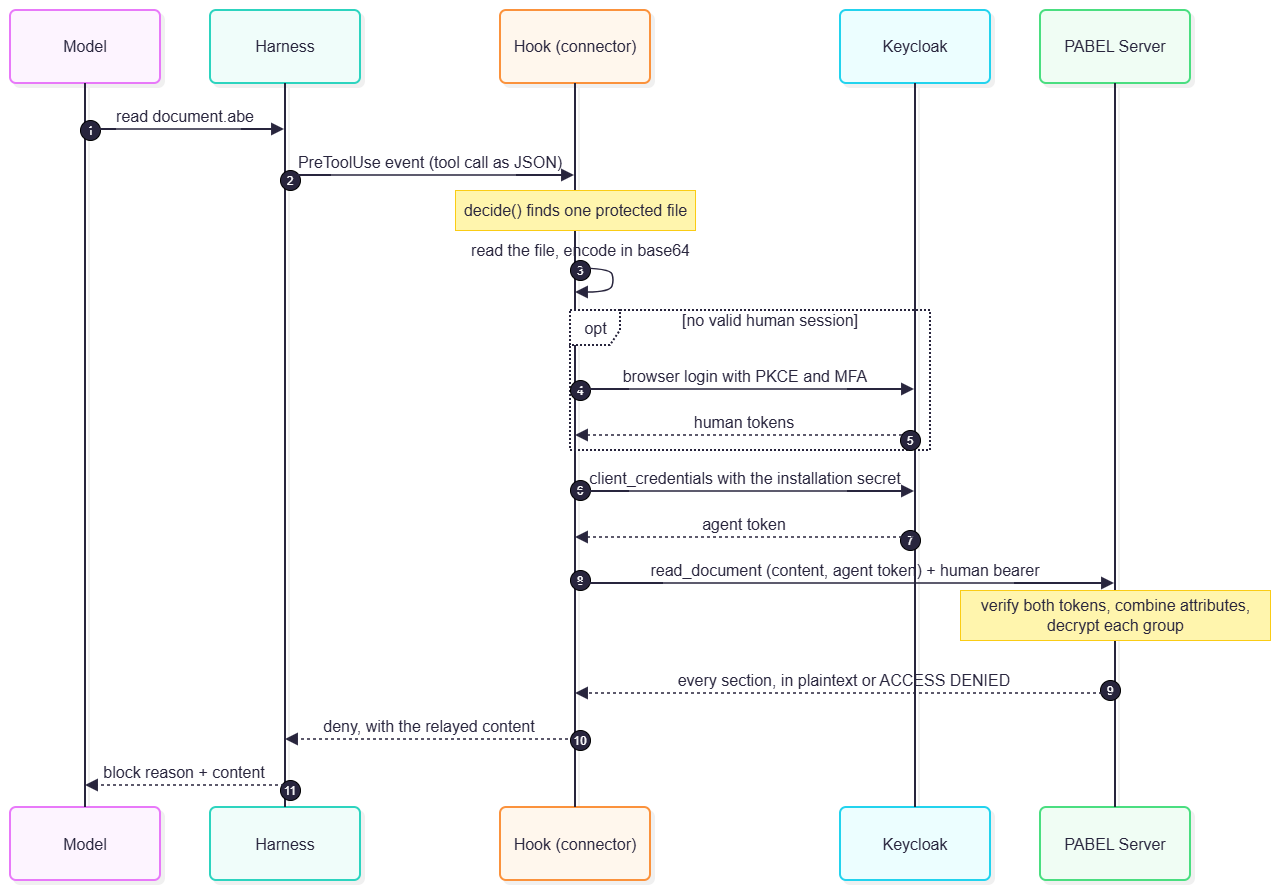
\includegraphics[width=\textwidth]{media/diagrams/Relay Hook flow.png}
  \caption{Flow of the relay of a protected read}\label{fig:relay}
\end{figure}
\paragraph{Direct tool calls}
The hook is not the only path. The connector registers the MCP server which offers \code{whoami}, \code{read\_document}, \code{login} and \code{materialize\_document} as ordinary tools.
Those are the main function that every harness, even those without hooks (see Section \ref{Two Classes of Agents}), uses to provide functionalities.
In case of a harness with hooks, calls to the tools are allowed after it has injected the token of the installation into their arguments, so that the model never has to hold or manage it.

\paragraph{Local copies}
When a copy of a document is requested, \code{materialize\_document} writes the recieved content into a local cache. In case of a PDF (or any file, for the matter), it is rebuilt from the single parts that are returned omitting, or (if the user requested it) marking as "ACCESS DENIED", the denied sections.
The server's output does not obfuscate the denied parts, it never sends them.

From the moment the document is given, PABEL no longer governs it, which is why the copy is deleted when the session ends, bounding the exposure to one session (see Asssumptions in section \ref{Assumptions}).
\textbf{N.B.} the deletion is implemented for the harnesses that offer a session-end hook, such as currently Claude Code.

\subsubsection{Per-Agent Adapters}
Since each agent has its own way to be controlled, it is necessary to create a specific adapter for each one of them. The adapter is the component that will translate the generic workflow into agent-specific ones.
The general approach is to fold the content of the decision into the agent's reasoning process, so that if the decision is rejected, or better, if there is a deny from the \code{core.decide} function, then the agent will not be able to access the document and so it will not be able to use it in its reasoning process.
This is important because each and every agent has its own way to reason and use hooks, for example, Claude code uses \code{decision.updated\_input}, thanks to which the token of the installation can be injected in the direct call to the tools of the server; different story is for Copilot CLI we cannot fully rely to \code{additionalContext}.

Table \ref{tab:channels} summarises, for each harness, how a denial travels back to the agent and where the relayed content lands.

\begin{table}[htbp]
  \centering
  \begingroup\linespread{1.0}\small
  \begin{tabular}{@{}>{\raggedright\arraybackslash}p{0.22\textwidth}>{\raggedright\arraybackslash}p{0.34\textwidth}>{\raggedright\arraybackslash}p{0.38\textwidth}@{}}
    \toprule
    \textbf{Harness} & \textbf{Blocking channel} & \textbf{Content channel} \\
    \midrule
    Claude Code & \code{permissionDecision} & \code{additionalContext} \\ \hline
    OpenCode & exception thrown from \code{tool.execute.before} & folded into thrown message \\ \hline
    Copilot (VS Code) & \code{permissionDecision} & \code{additionalContext} \\ \hline
    Copilot CLI & \code{permissionDecision} & folded into \code{permissionDecisionReason} (\code{additionalContext} is unreliable) \\ \hline
    Cursor & \code{permission}: alow, deny or ask & \code{agent\_message} \\ \hline
    Codex CLI, ChatGPT desktop & none (no hook) & none \\
    \bottomrule
  \end{tabular}
  \endgroup
  \caption{How each harness receives the denial and the relayed content}\label{tab:channels}
\end{table}

Following we can see fragments of those two implementations for Claude code and Copilot CLI, respectively:
\begin{lstlisting}[language=Python, caption={Claude code adapter}]
def render(decision: Decision) -> RenderedResponse:
    if decision.kind == DecisionKind.ALLOW:
        if decision.updated_input is None:
            return RenderedResponse()  # no output at all - the tool call proceeds untouched
        # A direct call to pabel's own tools, allowed through with this
        # installation's agent credential injected - see core/decide.py.
        return RenderedResponse(stdout=json.dumps({
            "hookSpecificOutput": {
                "hookEventName": "PreToolUse",
                "permissionDecision": "allow",
                "updatedInput": decision.updated_input,
            }
        }))

    output = {
        "hookSpecificOutput": {
            "hookEventName": "PreToolUse",
            "permissionDecision": "deny",
            "permissionDecisionReason": decision.reason,
        }
    }
    if decision.content is not None:
        output["hookSpecificOutput"]["additionalContext"] = json.dumps(decision.content)
    return RenderedResponse(stdout=json.dumps(output))
\end{lstlisting}
\begin{lstlisting}[language=Python, caption={Copilot CLI adapter}]
def render(decision: Decision) -> RenderedResponse:
    if decision.kind == DecisionKind.ALLOW:
        return RenderedResponse()

    # The guaranteed channel: fold the relay result into the reason text
    # itself, since additionalContext delivery is unreliable here.
    reason = fold_content_into_reason(decision)
    output = {
        "hookSpecificOutput": {
            "hookEventName": "preToolUse",
            "permissionDecision": "deny",
            "permissionDecisionReason": reason,
        }
    }
    if decision.content is not None:
        output["hookSpecificOutput"]["additionalContext"] = json.dumps(decision.content)
    return RenderedResponse(stdout=json.dumps(output))
\end{lstlisting}
\subsubsection{Two Classes of Agents}\label{Two Classes of Agents}
Agents differ on what their harness lets us control and this splits them into two categories:
\begin{itemize}
  \item \textbf{Interceptable agents}, which expose a hook that the runtime executes before a toll call; a direct read of a protected file can be blocked and replaced by the relayed, access-controlled result, without the model's intervention. Two example are Claude Code and OpenCode.
  \item \textbf{MCP-only agents}, i.e. agents that provide no interception mechanism. PABEL tools are registered as ordinary MCP tools that the model is free to call or not. They are accompanied by an informational skill, which is guidance and not an enforcement.
\end{itemize}
It is important to state what this distinction does \textit{not} change, in fact, a protected file is encrypted in both cases, so its confidentiality does not depend on the hook.

What the hook really adds is the impossibility to bypass the workflow, for example, by reaching the credential store, rewriting the hook configuration, invoking the OpenABE binaries directly (if available) or even lying about the agent's own identity.
For an MCP-only agent these protections are not available and the agent is simply a client for the server like any other.

The status of each harness is reported in Section \ref{Evaluation}
\subsection{Document Lifecycle}
The document starts its life whenever it is created and encrypted by somenoe, say a manager, that has to include sensitive information in said document.
Once the appropriate policy is defined and used to encrypt the document, it is stored (on the endpoint or in a central storage) and it become available through requst at the MCP server.
The document itself in our demo is stored directly on the client machine, but future developments could also lead to a centralized storage (see \nameref{Future Development}).

\begin{figure}[h]
  \centering
  
\includegraphics[width=\textwidth]{media/diagrams/Document Lifecycle.png}
  \caption{The flow diagram of the document lifecycle}
\end{figure}

When an agent requests access to a document, the hook will intercept the request and will start the authentication, first of the user and then of the agent. Everything is used to evaluate the CP-ABE policy and, if the user and the agent are both allowed to access the document, then the decryption will be performed and the document will be sent back to the agent; if not, the request will be denied and the agent will not have access to the document.


\subsection{Deployment Architecture}
We hereby explain how the architecture is topologically composed and, more in detail, where each component stores its data.
\subsubsection{Topology}
PABEL is deployed on two kinds of machines: the \textbf{server host} and the \textbf{employee machine}. The first one runs three containers (Keycloak, PostgreSQL, MCP server) orchestrated with \code{nerdctl compose} on Rancher Desktop and it is managed by an admin, the second one runs the agent alongside the connector (hook, adapters and local credential store).
The system was also tested with server and client on two different machines.
\begin{figure}[H]
  \centering
  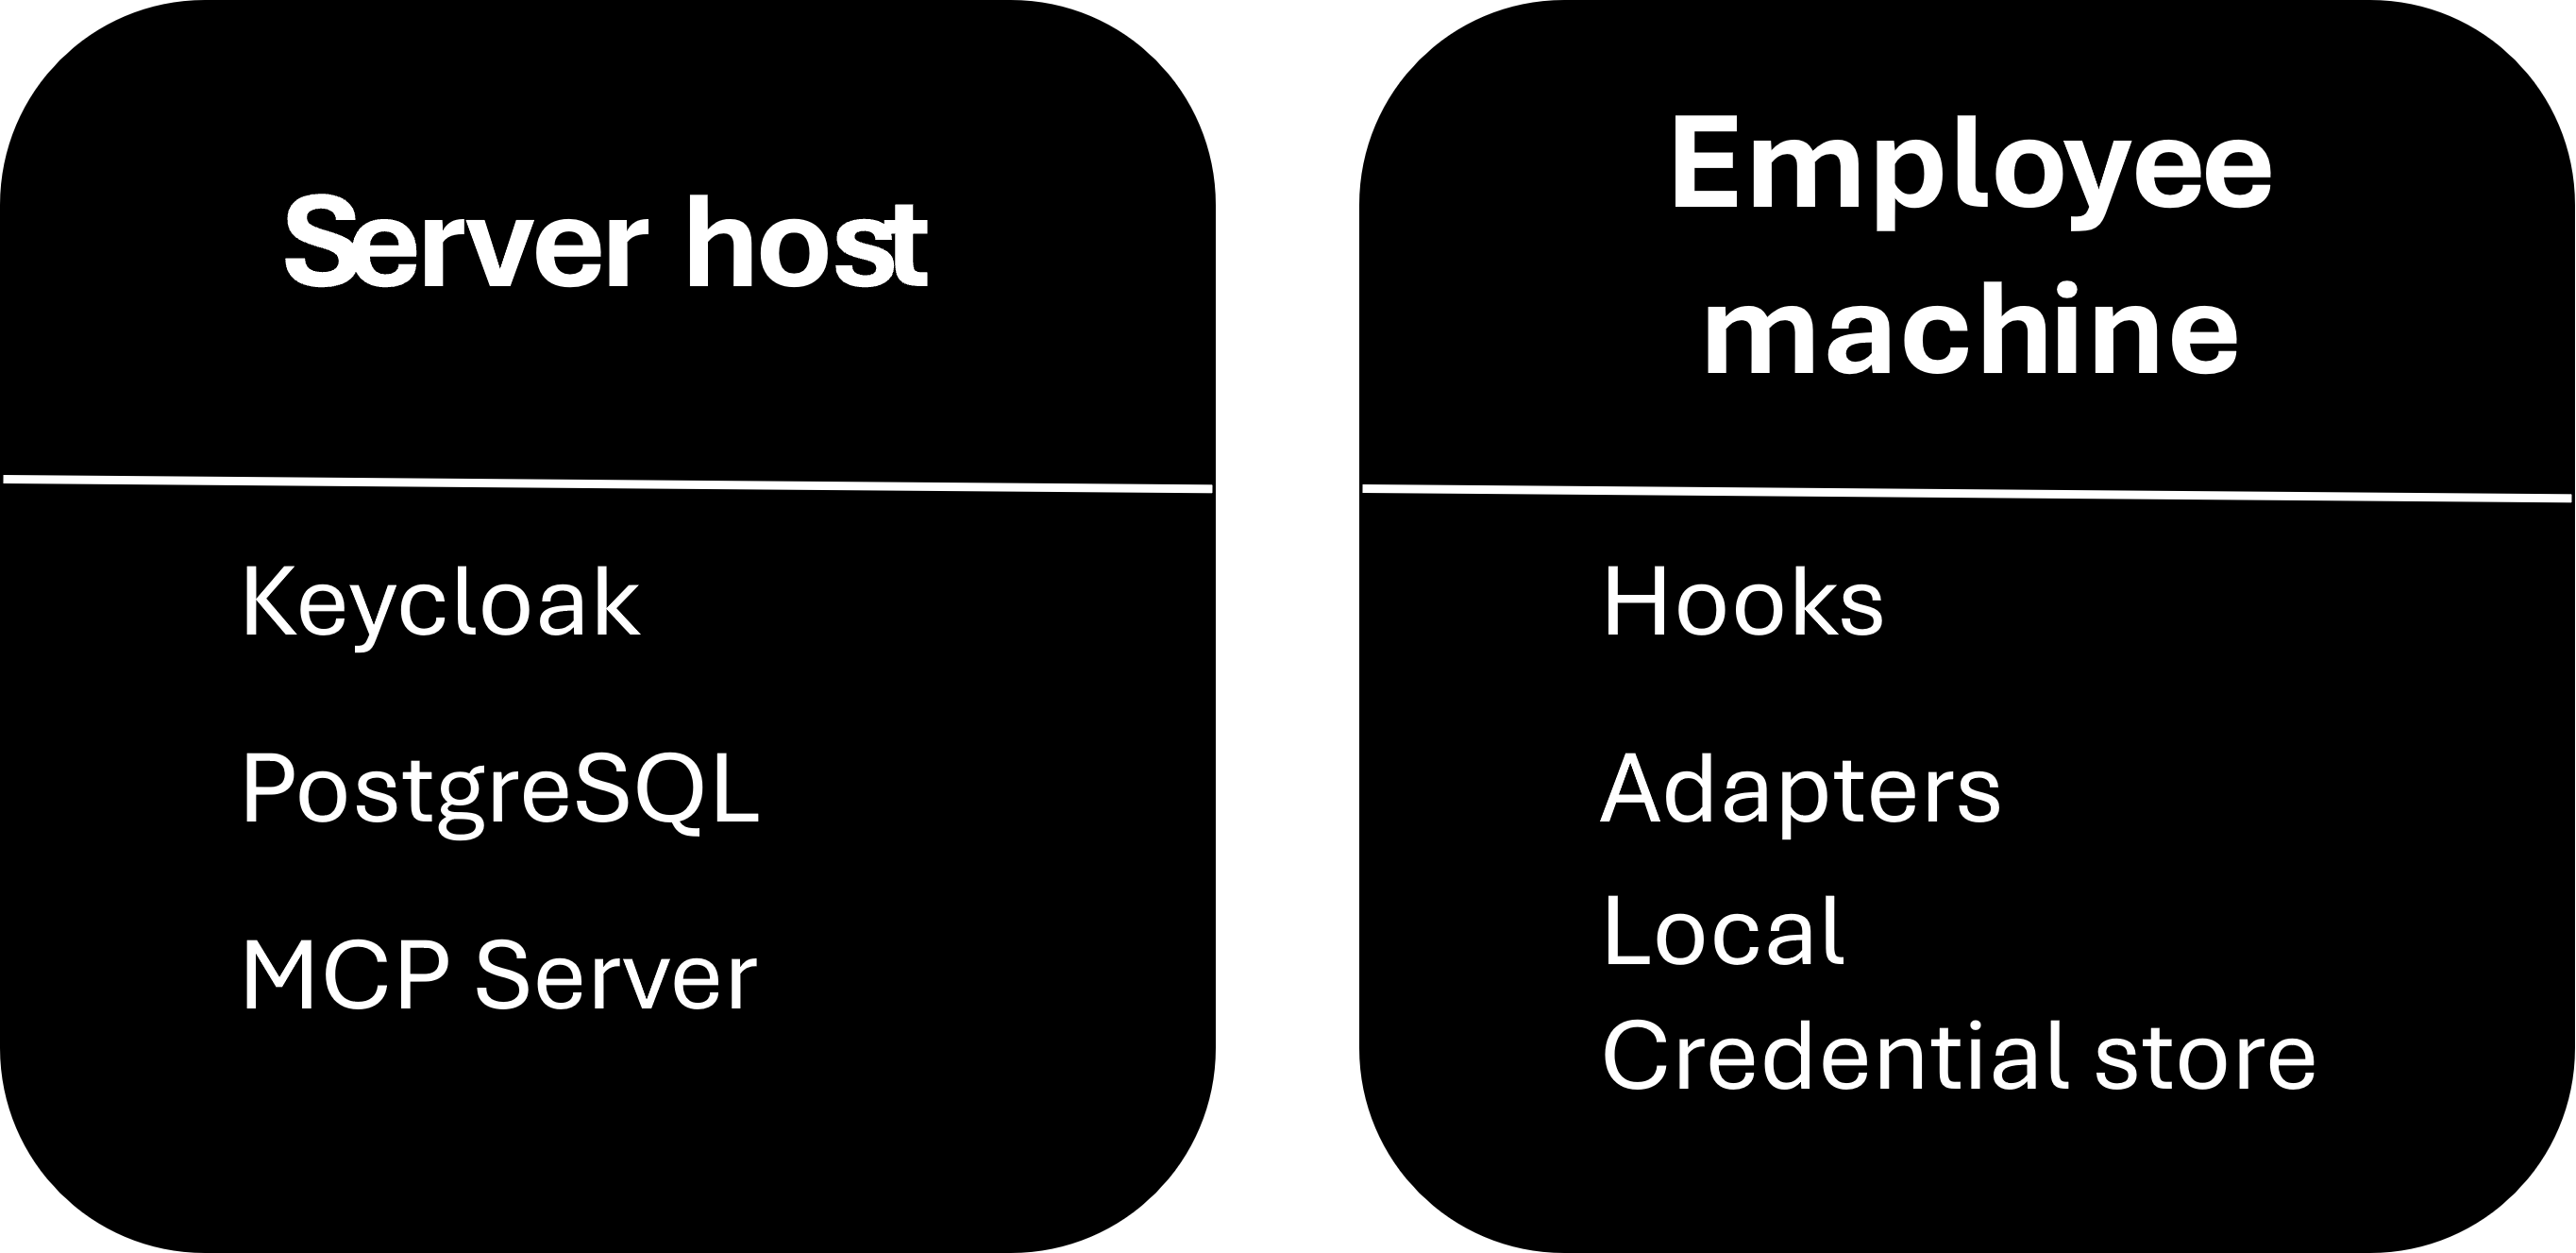
\includegraphics[width=0.8\textwidth]{media/image/Machine dichotomy.png}
  \caption{The two types of machines}
\end{figure}
It is worth note that only the container with the MCP server holds the CP-ABE authority (the master secret key) and each employee machine reaches the server over the network.

\subsubsection{Location of Each Component}
The following table (Table \ref{tab:state}) lists, for each component, the state it holds and where.

\begin{table}[htbp]
  \centering
  \begingroup\linespread{1.0}\small
  \begin{tabular}{@{}>{\raggedright\arraybackslash}p{0.17\textwidth}>{\raggedright\arraybackslash}p{0.17\textwidth}>{\raggedright\arraybackslash}p{0.33\textwidth}>{\raggedright\arraybackslash}p{0.23\textwidth}@{}}
    \toprule
    \textbf{Component} & \textbf{Runs on} & \textbf{State} & \textbf{Persistence} \\
    \midrule
    Keycloak & server host & users, attributes, roles, agent clients & inside the container, no volume \\
    PostgreSQL & server host & \code{agents}, \code{agent\_installations}, \code{agent\_keys}, \code{audit\_log} & volume \code{pgdata} \\
    MCP server & server host & master public and secret keys, \code{audit.jsonl} & bind mounts \code{authority} and \code{state} \\
    Connector & employee machine & agent credential, human session & user directory \code{\textasciitilde/.pabel/} \\
    \bottomrule    
  \end{tabular}
  \endgroup
  \caption{State held by each component and where it is stored}\label{tab:state}
\end{table}
\newpage
\section{Security Analysis}\label{Security Analysis}
Will follow an in depth analysis of each threat previously mentioned in the threat model after a breaf explanation of the security properties of our system.
Each subsection will explain for each threat the scenario and its causes, providing also the consequent residual risk.

\begin{table}[H]
    \centering
    \begin{tabular}[c]{|>{\raggedright\arraybackslash}m{0.3\textwidth}|>{\raggedright\arraybackslash}m{0.3\textwidth}|>{\raggedright\arraybackslash}m{0.3\textwidth}|}
        \hline
        \textit{\textbf{Threat}} & \textit{\textbf{Attack Goal}}       & \textit{\textbf{PABEL Mitigation}}   \\ \hline
        Unauthorized user        & Read protected data                 & Human authentication + ABE           \\ \hline
        Unauthorized agent       & Read protected data                 & Agent identity + ABE                 \\ \hline
        User / Agent mismatch    & Bypass policy                       & Combined attributes                  \\ \hline
        Agent Impersonation      & Fake agent identity                 & Installation credentials             \\ \hline
        Prompt injection         & Trick agent into requesting secrets & Interception + authorization         \\ \hline
        Network attacker         & Steal / forge traffic               & \raggedright Token verification + TLS {[}+ VPN{]} (see Section \ref{Future Development})\arraybackslash \\ \hline
        Compromised endpoint     & Read plaintext                      & Out of scope                         \\ \hline
        Master Key compromise    & Decrypt everything                  & Operational key protection           \\ \hline
        Post-decryption leakage  & Exfiltrate plaintext                & Out of scope / limitation            \\ \hline
    \end{tabular}
    \caption{Summary of various possible threat scenarios}
\end{table}

\subsection{Security Properties}
It is important to note, that the analysis refers to five properties of the system:
\begin{enumerate}
  \item[\textbf{P1}] \textbf{Two authentication, on every call.} The human and the agent are verified on every request; nothing is kept as ``logged in''.
  \item[\textbf{P2}] \textbf{Cryptographic, per-section enforcement.} A section opens only if the combined key satisfies its policy; the server does not filter, it is unable to open the others.
  \item[\textbf{P3}] \textbf{No key or credential at the agent.} Keys stay on the server and, for harnesses with a hook, the credentials of the installation are injected by the hook and are not readable by the model.
  \item[\textbf{P4}] \textbf{Accountability.} Every call that reaches the server leaves a record with user, agent and outcome.
  \item[\textbf{P5}] \textbf{Fail-closed interception.} Once the hook runs and there is an authentication or relay's error, it all ends in a denial and never in a direct read.
\end{enumerate}

\subsection{Unauthorized User}
The attacker is a person who holds no attribute that satisfies the policy of a section; it can be an employee outside the required department or even an outsider with a stolen password.
They could try to obtain a token without the 2FA, but the only way to login is the Authorization Code flow that is hosted by the identity provider and PABEL's client doesn't enable direct password grant, so any attempt without the 2FA authorized by the realm is uneffective.

An attacker could also attempt to raise its own attributes, but those fed a key that can only be edited by an administrator, never by a user.
Even a forged token wouldn't work, since the server verifies its signature against the keys published by the realm and also its issuer and expiration.

Finaly, a malevolent actor could try to directly read the file, but everything sensible is in form of a ciphertext, hence the cryptography is the security measure.
No key without the correct attributes satisfies a given policy, thus cannot decrypt it \cite{bethencourt2007ciphertext}: the denial does not rest on a check that could be skipped.

\paragraph{Residual risk} A user is, by design, able to read what their attributes allow and what they do with it is addressed in section \ref{sec:postdecryption}.

\subsection{Unauthorized Agent}
The attacker is an agent that the organization has not approved, or an apporved one that must not serve a given user.
An installation that is unknown, revoked or belonging to a disabled product will always fail the verification and the request will be denied.
In case of a valid installation, but used by someone not intended or simply wihtout the role required by its product is not rejected, but instead is treate like it has no attributes, thus every section which name the agent will stay close.

\paragraph{Residual risk} The consequences of this design must be kept in mind by who writes the policies.
A section whose policy does not name any agent is satisfied by the user alone through \textit{any} recognized installation.
Restricting a section to some agents is done by naming them in its policy and restricting \textit{any} agent by defining an unobtainable attribute (e.g. say "\code{no-agent}" that will not be addressed to any agent, see section \ref{CPvsKP}).

\subsection{User-Agent Collusion}
In this scenario the attacker is a user who handles an agent, possibly one under their control, and tries to obtain together more than each of them is entitled to.
The key used in a request is built for one pair and it carries exactly the union of the attributes of both user and installation in use. A section whose policy requires both, such as \code{sales and agent\_claude\_code}, opens for that pair and this is the intended meaning of the policy rather than a leak.
The structure itself is anti-collusion, i.e. nothing in the pair can add attributes that neither holds.

It is important to underline that even a user with two installations cannot merge them, since a request uses only one of them and having one with two agents would never be satisfied.

\subsection{Prompt Injection}
Content processed by the agent (a page, a file, the output of a tool, etc...) carries instruction that do not correspont to the ones of the user (e.g. read a protected document, obtain credential, disable enforcement, etc...).

An attacker could controls the content but nothing else, neither the machine nor the tokens.
They could ask ultimately three things:
\begin{enumerate}
    \item An attacker could ask for a document the user cannot read: this fails since the key is determined by the authenticated identities of user and installation, not by anything written in a prompt;
    \item It could be ask to obtain credential or to disable the enforcement, but here the hook denies the request and it is not part of the reasoning of the model, hence it decides on the shape of the call (see Table \ref{tab:decide});
    \item Lastly, an injection could try to read something that the user is entitled to read, but any mechanism of the system prevents that (see Section \ref{sec:postdecryption}).
\end{enumerate}
\paragraph{Residual risk} For agents without hooks the second scenario is not blocked and the risk actually resides in the fact that installations are not shielded from the model (Section \ref{Two Classes of Agents}), still keeping the security assurances given by the cryptography, since protected files remain ciphertext.

\subsection{Agent Impersonation}\label{sec:impersonation}
A compromised or manipulated agent tries to act as another installation, to obtain the attributes of a more privileged harness.
The identity of the agent is the verified \code{azp} claim of a token that Keycloak issued, never a value the caller declares (Section \ref{Agent Identity Model}).
On the "hooked client", the hook denies the two routes that would let the model choose an identity, that is rewriting the configuration (\code{DENY\_CONFIG\_TAMPER}) or invoking the functionalities directly with a chosen agent (\code{DENY\_HOOK\_BYPASS}).

The second denial was added after a live session of GitHub Copilot. It was observed that it was calling the relay from a shell command with the identifier of another harness, to "borrow" its credential.
\paragraph{Residual risk} The credential of an installation is stored in a directory of the client machine. For harnesses with hooks the model cannot read it, for MCP-only harnesses this protection does not exist. A stolen credential could be revoked by flagging as such said installation.

\subsection{Credential Theft}
The objects worth stealing are three: human's session, installation's secret and the keys cached in the database.
Any of these, singularly taken, is not enough to read a protected document.
An attacker, with only a user token could obtain a key that lacks the attributes of the agent, thus every section tied to a specific agent stays closed; vice versa if an attacker has only an installation token it will still require a human login with 2FA.
In any case tokens have a limited lifetime, furthermore, an installation can be revoked simply fagging it and a user could be easily disabled by the identity provider.

\paragraph{Residual risk} The cached keys are decryption keys: whoever holds them can decrypt offline whatever attributes they satisfy, althoudh they cannot generate other keys.
\textbf{N.B.} In this work, both keys and secrets are on the client machine with no further protection (see Section \ref{Future Development}).

\subsection{Network Attacker}
An attacker observes or modifies the traffic between client and server.
Forging a request does not work because a token whose signature, issuer and expiration do not check is rejected.
Even intercepting the authorization code in the redirect towards the local machine is of no use without the verifier, which is never sent with the code \cite{rfc7636}.

\paragraph{Residual risk} The response of the server carries the plaintext of each section the pair may read and a bearer token can be replayed by whoever observes it during its validity.
Those issues can be mitigated via encryption and confining the system inside a VPN (see Section \ref{Future Development}).

\subsection{Compromised Endpoint}
An attacker who controls the client machine, act with the privileges of its user, so he can remove or bypass the hook and read the credentials stored there.
This scenario, however, is declared out of scope in the adversary model (Section \ref{Motivation and Threat Model}).
The consequences are nevertheless bounded, since document not yet read are still ciphertext and the server applies the same checks to every call, thus the attacker gets at most what the stolen identities allow.

\subsection{Master Key Compromise}
Whoever holds the master secret key can generate a key for any set of attributes and no policy could resist them: the authority is the root of trust of the whole system (Section \ref{Background}).
Ideally, the key is created inside the server, never sent elsewhere and used only by the server itself whithin the scope of the authoring tool.
Its custody is assumed in the threat model (Section \ref{Motivation and Threat Model}) and the only remedy to such scenario is a new authority that would make previous encrypted document unreadable.

\subsection{Post-Decryption Leakage}\label{sec:postdecryption}
When the server outputs the decrypted data to the agent, the guarantees of PABEL end (as shown in Figure \ref{fig:boundary}).
The agent, its vendor, the user or an injected instruction can send them anywhere and no application-level mechanism can prevent it.
What the system offers is minimization and accountability: only the sections that the user and the agent are entitled to are released, not the whole document; every release is recorded with the number of readable sections and the copies explicitly requested are deleted at the end of the session via session-end hook.
\begin{figure}[H]
    \centering
    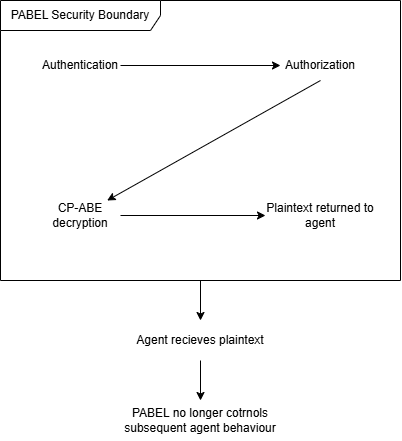
\includegraphics[width=0.8\textwidth]{media/diagrams/Security Boundary.png}
    \caption{PABEL's security boundary}\label{fig:boundary}
\end{figure}
\paragraph{Residual risk} The data exposed to the vendor is exactly the data the policy allows and no more; what the vendor, the model or the user does with it is outside the control of this work.

\subsection{Limitations}
Several limitations of this work, notably the unencrypted transport, the protection of keys and secrets at rest and the verification of the audience of the tokens, are listed in Table~\ref{tab:target} together with the deployment they are expected to reach (Section~\ref{Future Development}).
Other limitations that belong to the design are:
\begin{itemize}
  \item The interception is as strong as the hook: a user can theoretically remove it, a harness without hooks is not enforced and where the wiring is missing the read is not intercepted, although the file remains ciphertext.
  \item The local log of the connector records the outcomes for a third party who later obtains it, but it cannot protect against the agent it records; the trail of the server is the record, and it covers only the calls that reach the server.
  \item A single authority holds the master key and replacing it invalidates every existing document.
  \item Only the harness is identified, never the model and the enforcement operates at the application level.
  \item A policy that does not name an agent is satisfied by any recognised installation.
\end{itemize}

\newpage
\section{Evaluation}\label{Evaluation}
\subsection{Evaluation Goals}
This section will focus on the evaluation done throughout this work.
The main question we want to address are:
\begin{itemize}
  \item Does the system give exactly the sections the corresponding policy allows?
  \item Does the system resist the attacks defined in the threat model (Section \ref{Motivation and Threat Model})?
  \item How mnay resources the system uses?
  \item Does the system works on a single machine with more than one agent?
\end{itemize}
Each of those questions is addressed in the following subsections.

\subsection{Experimental Setup}
Before presenting the observed results, we present to the reader how the system is setup.

All of the tests are run in a single machine that host multiple containers for the server-side components and multiple client installation for each agent on said machine.
Claude Code and OpenCode are the most used agents, but we mention also Codex and Copilot as alternatives tried in some tests.

Documents were built purposely with ABEditor (see Section \ref{ABEditor}), which also provides the expected outcome for each section.
It is also important to note that we have used fictitious users defined with their own attributes as following:

\begin{table}[H]
  \centering
  \begin{tabular}{lll}
    \toprule
    \textbf{User} & \textbf{ABE Attributes} & \textbf{Agents allowed (role)} \\
    \midrule
    alice & ceo, executive, security  & Claude Code, opencode \\
    bob & hr, sales, marketing  & Claude Code \\
    charlie & dev, risk, executive  & opencode \\
    \bottomrule
  \end{tabular}
  \caption{Fictitious users: attributes (claim \code{abe\_attributes}) and agents roles defined in this realm.}\label{tab:eval-users}
\end{table}

\subsection{Automated Tests}
Table \ref{tab:eval-unit} lists the 258 automated tests by area. They do not need neither containers, nor database, nor OpenABE, htey tests the actual code, i.e. the decision logic, the agent adapters, the installers and the client.

% ---------------------------------------------------------------- unit tests
\begin{table}[H]
  \centering
  \begingroup\linespread{1.0}\small
  \begin{tabular}{@{}l>{\raggedright\arraybackslash}p{0.6\textwidth}r@{}}
    \toprule
    \textbf{Suite} & \textbf{Area} & \textbf{Tests} \\
    \midrule
    connector & Detection and decision (\code{decide}, \code{detection}, \code{hook}) & 60 \\
    connector & Agent adapters                                                         & 37 \\
    connector & Installers and CLI (\code{install}, \code{doctor}, \code{global}, managed settings) & 89 \\
    connector & Client (relay, sessions, local audit log, materialize, recompose, local MCP) & 48 \\
    server    & Document model, agent resolution, audit and keys, \code{.abe} line endings & 24 \\
    \midrule
    \multicolumn{2}{@{}l}{\textbf{Total}} & \textbf{258} \\
    \bottomrule
  \end{tabular}
  \endgroup
  \caption{Automated tests by area: 258 tests, 257 pass and 1 skipped because \code{pymupdf} is not installed. None of them needs a container, a database or OpenABE.}\label{tab:eval-unit}
\end{table}

\subsection{Functional Correctness}
Each document was opened by every user-agent pair and for each section the observed outcome was compared with the one expected from its policy and from the attributes of the pair.
Table \ref{tab:eval-matrix} reports the number of readable sections.

The same user obtains different sections through different agents (e.g. alice: 3/3 with Claude Code, 2/3 with opencode) and an installation used without its role is recognized but recieves no agent attributes (e.g. bob with opencode).

Reads recorded during development (Table \ref{tab:eval-audit}) show the same pattern, but they come from usage and not from a controlled experiment.

\begin{table}[H]
  \centering
  \begingroup\linespread{1.0}\small
  \begin{tabular}{@{}>{\raggedright\arraybackslash}m{0.14\textwidth}>{\raggedright\arraybackslash}m{0.18\textwidth}>{\raggedright\arraybackslash}m{0.22\textwidth}>{\raggedright\arraybackslash}m{0.22\textwidth}>{\raggedright\arraybackslash}m{0.12\textwidth}@{}}
    \toprule
    \textbf{User} & \textbf{Agent} & \textbf{Expected (ABEditor)} & \textbf{Observed (PABEL)} & \textbf{Result} \\
    \midrule
    alice & claude-code & 3/3 & 3/3 & pass \\
    alice & opencode    & 2/3 & 2/3 & pass \\
    bob   & claude-code & 2/3 & 2/3 & pass \\
    \bottomrule
  \end{tabular}
  \endgroup
  \caption{Readable sections per user--agent pair on a purpose-built document of three sections: outcome expected from the policies and outcome observed through PABEL.}\label{tab:eval-matrix}
\end{table}

% ---------------------------------------------------------------- audit
\begin{table}[H]
  \centering
  \begingroup\linespread{1.0}\small
  \begin{tabular}{@{}rllrr@{}}
    \toprule
    \textbf{Sections} & \textbf{User} & \textbf{Agent} & \textbf{Readable} & \textbf{Runs} \\
    \midrule
    3  & alice   & opencode        & 2/3   & 2 \\
    3  & alice   & vscode          & 0/3   & 2 \\
    3  & charlie & chatgpt-desktop & 1/3   & 2 \\
    4  & alice   & opencode        & 3/4   & 2 \\
    4  & bob     & claude-code     & 3/4   & 2 \\
    39 & alice   & claude-code     & 17/39 & 4 \\
    39 & alice   & opencode        & 5/39  & 3 \\
    39 & charlie & opencode        & 18/39 & 2 \\
    \bottomrule
  \end{tabular}
  \endgroup
  \caption{Reads recorded in the server audit log (\code{read\_document}, outcome ok) whose value was the same in at least two runs. Pairs that gave different values between runs (document or attributes changed) are left out: alice/claude-code and bob/opencode on 3 sections, bob/claude-code on 3 and 39 sections. The rows come from usage, not from a controlled experiment.}\label{tab:eval-audit}
\end{table}


\subsection{Security Tests}
The scenarios of Table \ref{tab:eval-security} were run through the real entry point of the hook, without a server and with fake credentials, so they test the interception and not the server.
Since they were written together with the rules, they are regression tests more than indepentent evidence. For this reason, the same attacks were repeated in a different way (Table \ref{tab:eval-probes}).

% ---------------------------------------------------------------- security
\begin{table}[H]
  \centering
  \begingroup\linespread{1.0}\small
  \begin{tabular}{@{}llcc@{}}
    \toprule
    \textbf{Threat} & \textbf{Scenarios} & \textbf{Run} & \textbf{Result} \\
    \midrule
    Unauthorized user (direct read, 5 tools)        & U1--U5 & 5 & 5 pass \\
    Prompt injection (folder enumeration)            & N1--N2 & 2 & 2 pass \\
    Tampering with a document                        & M1--M2 & 2 & 2 pass \\
    Credential theft                                 & K1--K4 & 4 & 4 pass \\
    Agent impersonation                              & I1--I5 & 5 & 5 pass \\
    Bypassing the server (\code{oabe\_*} binaries)   & O1--O2 & 2 & 2 pass \\
    Injection of the installation credential         & J1--J3 & 3 & 3 pass \\
    No false positives                               & A1--A4 & 4 & 4 pass \\
    \midrule
    \textbf{Total} & & \textbf{27} & \textbf{27 pass} \\
    \bottomrule
  \end{tabular}
  \endgroup
  \caption{Attack scenarios run through the real hook entry point, without a server and with fake credentials. In U1--U5 the plaintext of the document never appears in the output; in J2 an \code{agent\_token} forged by the model is replaced by the one of the installation.}\label{tab:eval-security}
\end{table}

None of the eight variants was blocked. The credential check compares the litteral path, so \code{\textasciitilde}, \code{\$HOME}, a search or a glob on the credential folder escape it.
The rules on \code{oabe\_*} binaries and on the connector modules, apply only to the \code{Bash} tool and the protection of the configuration only to \code{Write} and \code{Edit}.
These gaps do not expose protected documents, which remain ciphertext, nor allow acting alone as a user, because both principals are still required (Section \ref{Security Analysis}). They do show that the claim that the model cannot read the credential holds only for the literal path, and they are listed in Section \ref{Future Development}.

\begin{table}[H]
  \centering
  \begingroup\linespread{1.0}\small
  \begin{tabular}{@{}llc@{}}
    \toprule
    \textbf{ID} & \textbf{Variant} & \textbf{Result} \\
    \midrule
    E1 & \code{oabe\_dec} from the \code{PowerShell} tool                      & not blocked \\
    E2 & import of \code{pabel\_connector} from \code{PowerShell}              & not blocked \\
    E3 & \code{cat \textasciitilde/.pabel/agent\_credentials.json}             & not blocked \\
    E4 & \code{cat \$HOME/.pabel/session.json}                                 & not blocked \\
    E5 & \code{Grep} on the credential folder                                  & not blocked \\
    E6 & glob \code{.pabel\textbackslash*.json}                                & not blocked \\
    E7 & rewriting \code{.claude/settings.json} with a shell redirect          & not blocked \\
    E8 & rewriting \code{.claude/settings.json} from \code{PowerShell}         & not blocked \\
    \bottomrule
  \end{tabular}
  \endgroup
  \caption{Probes: the same attacks in a different shape, all of which should be denied. The hook answers \code{ALLOW}; the attacks were not executed. The credential check compares the literal path; \code{DENY\_OABE\_BINARY} and \code{DENY\_HOOK\_BYPASS} apply only to the \code{Bash} tool, and \code{DENY\_CONFIG\_TAMPER} only to \code{Write} and \code{Edit}.}\label{tab:eval-probes}
\end{table}


\subsection{Agent Coverage}

\begin{table}[H]
  \centering
  \begingroup\linespread{1.0}\small
  \begin{tabular}{@{}llll@{}}
    \toprule
    \textbf{Agent} & \textbf{Class} & \textbf{Interception} & \textbf{Server-side enforcement} \\
    \midrule
    Claude Code       & hook     & verified   & observed \\
    opencode          & hook     & verified   & observed \\
    Copilot (VS Code) & hook     & unreliable & observed (alice: 0/3) \\
    ChatGPT desktop   & MCP only & none       & observed (charlie: 1/3) \\
    \bottomrule
  \end{tabular}
  \endgroup
  \caption{Coverage by agent (classes in Section \ref{Two Classes of Agents}). The server applies the same checks to every agent, only the interception depends on the hooks of the harness. Server-side figures come from Table \ref{tab:eval-audit}.}\label{tab:eval-coverage}
\end{table}

\subsection{Performance}

\subsubsection{Format versions}
\subsubsection{Latency of a protected read}
\subsubsection{Cost of the hook}

% ---------------------------------------------------------------- performance
\begin{table}[H]
  \centering
  \begingroup\linespread{1.0}\small
  \begin{tabular}{@{}lrrr@{}}
    \toprule
    \textbf{Measure} & \textbf{Median (ms)} & \textbf{p95 (ms)} & \textbf{Runs} \\
    \midrule
    Python interpreter (\code{python -c pass})                 & 115  & 124  & 30 \\
    Loading the hook code                                       & 1307 & 1387 & 30 \\
    Hook on an unrelated call (\emph{allow})                    & 1312 & 1380 & 30 \\
    Hook on a local denial (\emph{deny})\textsuperscript{a}     & 1322 & 1418 & 30 \\
    \midrule
    Decision alone, in-process                                  & \multicolumn{3}{l}{0.038 ms per call (2000 iterations)} \\
    \bottomrule
  \end{tabular}
  \endgroup
  \caption{Cost of the hook, as wall-clock time of the whole process (3 warm-up runs discarded, measures interleaved). Loading the modules accounts for about 1.19 s: \code{mcp} alone takes 710 ms out of 1097 ms with \code{-X importtime}. \textsuperscript{a}Without the round trip to the server, capped at 3 s. The virtual environment sits inside OneDrive, so the absolute values depend on the machine.}\label{tab:eval-hook}
\end{table}

\subsection{Deployment on Two Machines}

\subsection{Case Study: Nexora Demo}

\subsection{Summary of the Results}

% ---------------------------------------------------------------- summary
\begin{table}[H]
  \centering
  \begingroup\linespread{1.0}\small
  \begin{tabular}{@{}lcl@{}}
    \toprule
    \textbf{Test} & \textbf{Run} & \textbf{Result} \\
    \midrule
    Automated tests (connector and server)      & 258 & 257 pass, 1 skipped \\
    Functional matrix (user--agent pairs)       & 3   & 3 pass \\
    Security scenarios (baseline)               & 27  & 27 pass \\
    Security scenarios (probes)                 & 8   & 0 blocked \\
    \bottomrule
  \end{tabular}
  \endgroup
  \caption{Summary of the tests run. The cost of the hook is reported in Table \ref{tab:eval-hook}.}\label{tab:eval-summary}
\end{table}

\subsection{Limits of the Evaluation}

\newpage
\section{Conclusions}\label{Conclusions}
\subsection{Summary}
This work remarks how every innovation comes with perplexities, expecially when talking about security and privacy.
It was clear from the beginning that there is a lack of measures to ensure data privacy and control over useful and powerful tools as LLMs and agents in general.

The observation that started this thesis, that is having zero trust for both AI agent and its vendor, remain an open problem for enterpries an private customer alike.
Is important to state the vendors should provide more measures to handle agents and preferrably standardize those in a way more advanced works could be based on a more model-agnostic approach.

Ultimately, the hope of this work is to offer a solution to one important problem like the confidentiality over our own machine that now more than ever needs to be protected not only from what lies over the internet and other devices, but also from the potential threat that come from within ourself.
\subsection{Results}
\subsection{Future Development}\label{Future Development}
The implementation described in this work is a proof of concept and some of its choices do not reflect the deployment envisaged for a real organization.

Ideally, network traffic will travel inside a VPN and documents will be able to be decrypted not only from a client machine, but they may be choosen directly from a server, say, via an identifier.

As per today, the distance from the target deployment is summarized in the following table.
\begin{table}[htbp]
  \centering
  \begingroup\linespread{1.0}\small
  \begin{tabular}{@{}>{\raggedright\arraybackslash}m{0.17\textwidth}>{\raggedright\arraybackslash}m{0.36\textwidth}>{\raggedright\arraybackslash}m{0.39\textwidth}@{}}
    \toprule
    \textbf{Area} & \textbf{Prototype} & \textbf{Target deployment} \\
    \midrule
    Network & HTTP on a local network, ports of the services published to the host & every component inside a VPN, TLS between components, database not exposed \\
    Documents & read from the client machine and sent with each request; the server keeps no store & kept on the endpoint or retrieved from a central store by identifier \\
    Keycloak & development mode, data inside the container & production mode with a persistent, backed-up database \\
    Tokens & signature, issuer and expiry are verified & audience binding as well, as required by the MCP authorization specification \\
    Keys at rest & user-agent keys cached in PostgreSQL & keys protected at rest \\
    Client secrets & stored in a user directory of the client & stored in the secret store of the operating system \\
    Client enforcement & hook per user; managed deployment only for Claude Code & managed deployment for every harness that supports it \\
    Key cache & purged by hand if the authority is replaced & invalidated automatically when the authority changes \\
    Audit & JSON lines and a PostgreSQL mirror, local log not tamper-proof & append-only central storage \\
    Local copies & deleted at the end of the session only for Claude Code & deleted for every harness, with a time-based cleanup where no session-end hook exists \\
    \bottomrule
  \end{tabular}
  \endgroup
  \caption{From the prototype to the target deployment}\label{tab:target}
\end{table}

In the target deployment the guarantees described in this work are expected to hold and so are the assumptions.
All future developments will surely increase the overall security and usability of this work.

\newpage
\section{Bibliography}
\printbibliography
\end{document}